\chapter{Moduli problems}
    \begin{abstract}
        
    \end{abstract}
    
    \minitoc

    \section{Moduli problems}

    \section{Examples}
        \subsection{Hilbert schemes}
        
        \subsection{Picard schemes}
            \subsubsection{Line bundles and Picard stacks}
                \begin{definition}[Line bundles] \label{def: line_bundles}
                    \noindent
                    \begin{enumerate}
                        \item \textbf{(Line bundles):} Let $\calY$ be a prestack on $\Cring^{\op}$. Then, a \textbf{line bundle on $\calY$} is a line object (also referred to as an invertible object) in the \textit{symmetric} monoidal category $\QCoh(\calY)$ of quasi-coherent modules on $\calY$ (cf. definition \ref{def: qcoh_def}). For the definition of line objects, see \cite{nlab:line_object}.
                        \item \textbf{(Picard groupoids):} 
                            \begin{enumerate}
                                \item \textbf{(Picard groups ...):} It is not hard to see that given any symmetric monoidal category such as that of quasi-coherent modules over a prestack, isomorphism classes of its line objects (which are non-trivial in general, since monoidal structures are only defined up to coherence isomorphisms) form a group where the multiplication is the monoidal structure. This group is known as the \textbf{Picard group}; we shall denote the Picard group of a prestack $\calY$ on $\Cring^{\op}$ by $\Pic^0(\calY)$. Also, note that Picard groups are trivially abelian.
                                \item \textbf{(... and to categorify them):} However, one might not be content with line bundles forming just a puny group. If that is indeed the case, allow us to introduce the all-new \textbf{weak Picard $2$-group}. The weak Picard $2$-group associated to a given prestack $\calY$ on $\Cring^{\op}$ is first and foremost the category internal to the category $\Grp$ of groups (which we note to have finite pullbacks; see definitions \ref{def: internal_categories} and \ref{remark: internal_categories_alt_def} for an explanation of why this is necessary), whose object of objects is $\Pic^0(\calY)$ and whose object of arrows is the automorphism group $\Aut\left(\Pic^0(\calY)\right)$, which we shall suggestively abbreviate by $\Pic^1(\calY)$:
                                    $$
                                        \begin{tikzcd}
                                        	{\Pic^1(\calY)} & {\Pic^0(\calY)} \\
                                        	{\Pic^0(\calY)}
                                        	\arrow["t"', from=1-1, to=2-1]
                                        	\arrow["s", from=1-1, to=1-2]
                                        \end{tikzcd}
                                    $$
                                Next, observe that the above internal category possesses a natural groupoid structure, owing to the fact that the object of arrows $\Pic^1(\calY)$ is a group (by construction!), which in particular means that every arrow in the internal category $(s, t)$ is invertible, and thus there exists an inversion map:
                                    $$i: \Pic^1(\calY) \to \Pic^1(\calY): \sigma \mapsto \sigma^{-1}$$
                                which trivially fits into the following commutative diagram in $\Grp$ (we shall let the reader check the commutativity of this diagram as an exercise):
                                    $$
                                        \begin{tikzcd}
                                        	{\Pic^1(\calY)} \\
                                        	& {\Pic^1(\calY)} & {\Pic^0(\calY)} \\
                                        	& {\Pic^0(\calY)}
                                        	\arrow["t", from=2-2, to=3-2]
                                        	\arrow["s"', from=2-2, to=2-3]
                                        	\arrow["i"{description}, from=1-1, to=2-2]
                                        	\arrow["s"', from=1-1, to=3-2]
                                        	\arrow["t", from=1-1, to=2-3]
                                        \end{tikzcd}
                                    $$
                                    
                                One important thing to note is that the weak Picard $2$-group $(s, t): \Pic^1(\calY) \toto \Pic^0(\calY)$ is precisely the \href{https://ncatlab.org/nlab/show/core}{\underline{core}} of the full subcategory of $\QCoh(\calY)$ spanned by line bundles, as the automorphisms on $\Pic^0(\calY)$ are precisely the isomorphisms between line bundles on $\calY$, and thus it is also a groupoid in the usual sense (i.e. a groupoid internal to $\Cat$). In particular, this tells us that the weak Picard $2$-group of a prestack is actually strict, and it is for this reason that sometimes we might confuse the terms \say{Picard $2$-group} and \say{Picard groupoid}.
                                
                                From this point on, the Picard $2$-group/groupoid associated to a given prestack $\calY$ shall be denoted simply by $\Pic^1(\calY)$.
                            \end{enumerate}
                    \end{enumerate}
                \end{definition}
                \begin{remark}[A categorical comment] \label{remark: picard_2_groups_are_groups_in_Cat}
                    Because Picard $2$-groups associated to prestacks are strict $2$-groups, they also enjoy the property of being group objects in $\Cat$ and hence in the full subcategory $\Grpd$ thereof. See \cite{nlab:strict_2-group} for more details.
                \end{remark}
                \begin{remark}[Picard groups, Picard $2$-groups, and higher homotopical fairy tales]
                    Fix a prestack $\calY$ on $\Cring^{\op}$.
                    \begin{enumerate}
                        \item \textbf{(Decategorifying Picard $2$-groups):} The underlying set of the Picard group $\Pic^0(\calY)$ can be thought of as the set of connected components of the groupoid $\Pic^1(\calY)$, i.e.:
                            $$\Pic^0(\calY) \cong \pi_0\Pic^1(\calY)$$
                        Intuitively, this should make sense, since the data specifying $\Pic^1(\calY)$ differ from that specifying $\Pic^0(\calY)$ only by the \say{looping} isomorphisms on line bundles on $\calY$, which means that the set of connected components of $\Pic^1(\calY)$ is just the \say{discrete} part, namely the underlying set of $\Pic^0(\calY)$. 
                        \item \textbf{(Higher Picard groups):} For each natural number $n$, let us define the Picard $(n + 1)$-group $\Pic^n(\calY)$ to be the strict $(n + 1)$-group $\Aut^n\left(\Pic^0(\calY)\right)$, where:
                            $$\Aut^n\left(\Pic^0(\calY)\right) \cong \Aut\left( \Aut\left( \cdots \Aut\left(\Pic^0(\calY)\right) \right) \right)$$
                        Of course, for all $r \leq n$, we have:
                            $$\Pic^r(\calY) \cong \pi_r\Pic^n(\calY)$$
                    \end{enumerate}
                \end{remark}
                
                \begin{theorem}[\textit{Hilberts Satz 90}] \label{theorem: hilbert_90}
                    Let $X$ be an arbitrary scheme. Then, one has the following isomorphism of abelian groups:
                        $$\Pic^0(X) \cong H^1_{\tau}(X, \G_m)$$
                    where $\tau \in \{\text{Zariski, smooth, \'etale, fppf}\}$.
                \end{theorem}
                    \begin{proof}
                        
                    \end{proof}
                
                \begin{definition}[Picard prestacks] \label{def: picard_prestacks}
                    Let $k$ be a base commutative ring. Then, let us define the \textbf{Picard stack over $\Spec k$} to be the \href{https://ncatlab.org/nlab/show/core}{\underline{core}} of the full substack:
                        $$\Pic^1: [\Spec k]^{\op} \to \Grpd$$
                    spanned by line bundles of the stack $\QCoh: [\Spec k]^{\op} \to \Cat$ of quasi-coherent modules on ${}^{k/}\Comm\Alg^{\op}$. That is to say, the Picard prestack associates to each prestack $\calY \in [\Spec k]$, the category $\Pic^1(\calY)$ is the core of the full subcategory of $\QCoh(\calY)$ spanned by line bundles, i.e. nothing but the Picard $2$-group on $\calY$ (cf. definition \ref{def: line_bundles}). Naturally, the Picard prestack is fibred in groupoids, and thus has a shot at being geometric. Also, it is evident that the Picard prestack is a gerbe (cf. convention \ref{conv: prestacks}).
                \end{definition}
            
            \subsubsection{Picard stacks of curves}
        
        \subsection{Moduli stacks of elliptic curves and of abelian varieties}
            \subsubsection{Moduli of elliptic curves}
                \paragraph{Elliptic curves and their moduli}
                    \begin{definition}[Moduli spaces of elliptic curves] \label{def: moduli_of_elliptic_curves} \index{Moduli space! of elliptic curves}
                        \noindent
                        \begin{enumerate}
                            \item \textbf{(Elliptic curves):} An \textbf{elliptic curve} over a given base scheme $B$ is an $B$-scheme:
                                $$E \to B$$
                            that satisfies the following properties:
                                \begin{itemize}
                                    \item $E$ is smooth, proper, and of relative dimension $1$ over $B$.
                                    \item The fibre of $E$ over any point $x \in |B|$ is a smooth, proper, of pure dimension $1$, and geometric connected over the residue field $\kappa_x$.
                                    \item $E$ is a \textit{group $B$-scheme} and as such admits a \textbf{distinguished section} $o_E: B \to E$ as its unit.
                                \end{itemize}
                            In other words, an elliptic curve is an abelian scheme of relative dimension $1$.
                            \item \textbf{(Moduli spaces of elliptic curves):} Over a base scheme $S$, the \textbf{moduli space of elliptic curves} is a prestack:
                                $$(\calM_{1, 1})_{/S}: \Sch_{/S}^{\op} \to \Grpd$$
                            which associates to each $S$-scheme $B$ the \textit{core} (i.e. the maximal subgroupoid) of the category of elliptic curves over $B$ (in the above sense), which we will denote simply by $(\calM_{1, 1})_{/S}(B)$. One thing to note is that the pullback of fibres is given by fibred products, which is to say, given an underlying morphism:
                                $$f: B \to B'$$
                            the pullback along $f$ of an elliptic curve $E' \to B'$ (denoted by $f^*E'$) shall be the elliptic $B$-curve fitting into the following pullback square:
                                $$
                                    \begin{tikzcd}
                                    	{f^*E'} & {E'} \\
                                    	B & {B'}
                                    	\arrow[from=1-1, to=2-1]
                                    	\arrow["f", from=2-1, to=2-2]
                                    	\arrow[from=1-2, to=2-2]
                                    	\arrow[from=1-1, to=1-2]
                                    	\arrow["\lrcorner"{anchor=center, pos=0.125}, draw=none, from=1-1, to=2-2]
                                    \end{tikzcd}
                                $$
                        \end{enumerate}
                    \end{definition}
                    \begin{remark}[A few supplementary technical comments] \label{remark: moduli_of_elliptic_curves_disambiguations}
                        \noindent
                        \begin{itemize}
                            \item \textbf{(Categories of elliptic curves):}
                                \begin{enumerate}
                                    \item \textbf{(Morphisms of elliptic curves):} Fix a base scheme $B$. If one is to use definition \ref{def: moduli_of_elliptic_curves} as one's starting notion of what it means for a scheme to be an elliptic curve, then the morphisms in the category $(\calM_{1, 1})_{/S}(B)$ of elliptic $B$-curves are going to be \textit{group $B$-scheme homomorphisms}:
                                        $$
                                            \begin{tikzcd}
                                            	{E_1} && {E_2} \\
                                            	& B
                                            	\arrow[from=1-3, to=2-2]
                                            	\arrow["\phi", from=1-1, to=1-3]
                                            	\arrow[from=1-1, to=2-2]
                                            \end{tikzcd}
                                        $$
                                    \item \textbf{(Pullbacks):} It is well-known that thanks to the fact that limits commute, any limit of a group $B$-scheme taken in the ambient category $\Sch_{/B}$ would remain a group $B$-scheme. Is the same true for elliptic $B$-curves ? 
                                    
                                    To answer this question, one needs to verify that smoothness, properness, the dimension of elliptic curves being $1$, as well as fibres being geometrically connected are all properties stable under (finite) pullbacks. This is rather trivial for smoothness (as well as for relative dimensions) and to a lesser extent, for properness as well (which we recall to be the same as being separated, of finite type, and universally closed), so let us focus on geometric connectedness.
                                    
                                    Recall first of all that a scheme over a field is geometrically connected if and only if the underlying topological space of any of its geometric fibres is connected.
                                \end{enumerate}
                            \item \textbf{(Group structure on elliptic curves):} 
                                \begin{itemize}
                                    \item \textbf{(Group law):} Because limits of group schemes (taken in the ambient category of schemes) are still group schemes, the distinguished section $o_E: B \to E$ of a relative elliptic curve degenerates to a rational point $o_{E_x}: \Spec \kappa_x \to E_x$ (more generally, pullbacks do not interfere with the group structure of an existing elliptic curve). This is the usual \say{point at infinity} or \say{unit point} of an elliptic curve over a field (the residue field $\kappa_x$ in this case).
                                    \item \textbf{(Connectedness is important):}
                                \end{itemize}
                        \end{itemize}
                    \end{remark}
                        
                \paragraph{Good and bad reductions}
                    \begin{definition}[Models] \label{def: local_models_of_varieties} \index{Model! of an algebraic scheme}
                        Let $R$ be a discrete valutation ring with fraction field $K$ and let $X$ be an algebraic scheme $\Spec K$ (i.e. a scheme of finite type over $\Spec K$); often, $X$ will be a variety instead of a mere algebraic scheme. A \textbf{model for $X$ over a $\Spec R$} is a \textit{flat} and of \textit{finite type} $\Spec R$-scheme $\bbX$ whose pullback along the canonical arrow $\Spec K \to \Spec R$ is (isomorphic to) $X$, i.e. one fitting into the following pullback square:
                            $$
                                \begin{tikzcd}
                                	X & \bbX \\
                                	{\Spec K} & {\Spec R}
                                	\arrow[from=1-1, to=2-1]
                                	\arrow[from=2-1, to=2-2]
                                	\arrow[from=1-2, to=2-2]
                                	\arrow[from=1-1, to=1-2]
                                	\arrow["\lrcorner"{anchor=center, pos=0.125}, draw=none, from=1-1, to=2-2]
                                \end{tikzcd}
                            $$
                        In other words, a model for an algebraic scheme $X$ over the field of fractions $K$ of some discrete valuation ring $R$ is just a scheme $\bbX$ over $\Spec R$ whose generic fibre is precisely $X$. 
                        
                        One can also impose adjectives such as \say{smooth}, \say{\'etale}, or \say{proper} onto models of algebraic schemes, as long as morphisms characterised by these adjectives are flat and of finite type. If $P$ is a property described by one such adjective, then we say that a model $\bbX \to \Spec R$ is $P$ if and only if the morphism $\bbX \to \Spec R$ is $P$.
                    \end{definition}
                
                    \begin{definition}[Good and bad reductions] \label{def: reductions}
                        Let $X$ be an algebraic scheme over the field of fractions $K$ of a discrete valuation ring $R$, and let $\varpi \in R$ be a uniformiser (i.e. a generator of the unique maximal ideal of $R$). 
                        \begin{enumerate}
                            \item \textbf{(Good/bad reductions):} A reduction modulo $\varpi$ (or in other terminologies, at place $\varpi$) of a model $\bbX \to \Spec R$ of $X$ is just the pullback along the canonical morphism $\Spec R/\varpi \to \Spec R$ of $\bbX \to \Spec R$. It is called \textbf{good} if it is smooth or \say{better} (for instance, \'etale fibres can be considered good reductions). Otherwise, it is called \textbf{bad}.
                            
                            One thing to note is that smooth models and better ones \textit{a priori} have good reductions, since smoothness (and say, \'etale-ness) is preserved under arbitrary base changes (cf. proposition \ref{prop: compositions_and_base_changes_of_smooth_morphisms} and corollary \ref{coro: compositions_and_base_changes_of_etale_morphisms}).
                            \item \textbf{(Places of reduction):} Let $\varpi$ be a generator of the unique and (necessarily) principal maximal ideal of the discrete valuation ring $R$ (or equivalently, denote the unique and principal maximal ideal of $R$ by $(\varpi)$). An algebraic $K$-scheme $X$ is said to have a \textbf{place $\varpi$ of good reduction} if and only if there exist an $R$-model $\bbX \to \Spec R$ of $X$ whose reduction modulo $\varpi$ is good. One might also phrase things geometrically and say that $X$ has good reduction at the closed point $\Spec R/\varpi$.
                            
                            $X$ is said to have a \textbf{place $\varpi$ of bad reduction} if and only if there does not exist an $R$-model $\bbX \to \Spec R$ of $X$ whose reduction modulo $\varpi$ is good (or equivalently, if and only if the reduction modulo $\varpi$ of all $R$-models of $X$ are bad).
                            
                            For more information on so-called \say{places} and prime ideals, see convention \ref{conv: places_and_primes}.
                        \end{enumerate}
                    \end{definition}
                    \begin{example}[Reduction modulo $p$ of curves over $\Q$]
                        Let $p$ be a prime, and note firstly that $\Z_{(p)}$ is a discrete valuation ring by virtue of being a local PID that is not a field; its unique maximal ideal is $(p)$ (and hence one can take $p$ to be a uniformiser), as every element that is not equivalent to $0$ modulo $p$ has already been made to be invertible in $\Z_{(p)}$. Let $X$ be a smooth projective curve over $\Spec \Q$, and let $\bbX_{(p)} \to \Spec \Z_{(p)}$ be a model of $X$ (due to the Fundamental Theorem of Arithmetic, $\Z_{(p)}$ is has $\Q$ as its field of fractions). Then, a reduction modulo $p$ of $X$ is nothing but a fibre product $\bbX_{(p)} \x_{\Spec \Z_{(p)}} \Spec \F_p$. 
                    \end{example}
                    \begin{remark}[Locality of reduction]
                        It is worth noting that a curve $X \to \Spec K$ having good reduction at a place $\varpi$ is a local phenomenon. That is to say, a curve may have good reductions at all places $\varpi$ (for instance, there might be curves over $\Q$ such that all of their $\Z_{(p)}$ possess good modulo $p$ reductions), but the equation defining said curve may be singular in some manner after reduction modulo $\varpi$. 
                    \end{remark}
                    
                    \begin{lemma}[Existence of smooth models]
                        Let $R$ be a discrete valuation ring with field of fraction $K$. Then, there exist a flat, of finite presentation, and proper $R$-model $\bbX$ for any smooth scheme $X$ over $\Spec K$.
                    \end{lemma}
                        \begin{proof}
                            
                        \end{proof}
                    
                    \begin{theorem}[Shimura '55]
                        Let $X$ be a smooth projective variety over $\Spec \Q$. Then $X$ has finitely many places of bad reduction. That is to say, there are only finitely many places $p$ at which the reduction modulo $p$ of a $\Z_{(p)}$-model of $X$ is bad.
                    \end{theorem}
                        \begin{proof}
                            
                        \end{proof}
                    \begin{example}
                        \noindent
                        \begin{enumerate}
                            \item \textbf{(A cubic curve with places of bad reduction):} Consider the cubic curve given by the polynomial equation $x^3 - y^2  - 2 = 0$ (or in other words, consider the variety $X := \Spec \frac{\Q[x, y]}{(x^3 - y^2)}$), which we note to be smooth over $\Q$. Let $\bbX_{(p)}$ be a model over $\Spec \Z_{(p)}$ of $X$. Then, reductions modulo $p$ of $\bbX_{(p)}$ will remain smooth (i.e. good) at all places except at $p = 2$, because:
                                $$x^3 - y^2 - 2 \equiv x^3 - y^2 \pmod{2}$$
                            meaning that the reduction modulo $2$ of $\bbX_{(2)}$ has a cusp at the origin, and at $p = 3$, since:
                                $$x^3 - y^2 - 2 \equiv (x - 2)^3 - y^2 \pmod{3}$$
                            meaning that the reduction modulo $3$ of $\bbX_{(3)}$ has a cusp at $(x, y) = (2, 0)$.
                            \item \textbf{(Reductions of $p$-adic elliptic curves \cite[Example 5.2]{silverman_elliptic_curves}):} Let $p \geq 5$ be a prime and let $E_1, E_2$ be elliptic curves over $\Q_p$ that are given by the equations:
                                $$x^3 + px^2 - y^2 + 1 = 0$$
                            and:
                                $$x^3 - y^2 + p = 0$$
                            We know from the previous example that the second curve is cuspidal at place $p$, so let us focus our attention on the first curve. Reducing modulo $p$ gives a curve determined by the following equation:
                                $$x^3 - y^2 + 1 = 0$$
                            which we note to be smooth, and thus the place $p$ is of good reduction. The assumption that our prime $p$ is larger than or equal to $5$ is crucial for $p$ to be a place of good reduction for $E_1$, because when $p = 2$ or $p = 3$, the equation of the curve obtained after reduction modulo $p$ will be:
                                $$\text{$x^3 - (y + 1)^2 = 0$ or $(x - 1)^3 - y^2 = 0$}$$
                            and both are cuspidal.
                            \\
                            Over $\Q_p(\sqrt[6]{p})$, however, the curve $E_2$ does have good reduction at $p$: by setting $x = \sqrt[3]{p} s$ and $y = \sqrt[2]{p} t$, one gets the following equivalent equation defining the curve $E_2$:
                                $$ps^3 - pt^2 + p = 0$$
                            which becomes the trivial equation $0 = 0$ after reduction modulo $p$. 
                            \item \textbf{(Reduction of smooth projective $p$-adic surfaces):} Let $p$ be an arbitrary prime, let $K$ be a $p$-adic field (i.e. a finite extension of $\Q_p$), and let $X$ be a conic bundle over $\P^1_K$ with four degenrate fibres. First of all, note that $X$ is a smooth projective variety over $\Spec K$ whose $\ell$-adic cohomologies (with $\ell$ any prime distinct from $p$) are all unramified (cf. definition \ref{def: ramification_indices}). Second of all, by being a conic bundle, $X$ is $\overline{K}$-birational to $\P^1_K$. 
                            \item \textbf{(Reduction of abelian varieties):} Let $A$ be an abelian variety over $\Spec \Q$ and let $p, \ell$ be distinct primes. Then, by \cite[Theorem 1.1.1]{conradbrinon}, there exists a $\Z_{(p)}$-model of $A$ with good reduction at $p$ if and only if the $\ell$-adic \'etale cohomologies of $A$ are all unramified at $p$. A special case of this phenomenon is theorem 7.1 of \cite{silverman_elliptic_curves}, which gives a criterion by N\'eron-Ogg-Shafarevich for when elliptic curves admits good reduction at $p$;  
                        \end{enumerate}
                    \end{example}
                    
                    \begin{remark}[Global models ?] \label{remark: global_models}
                        Let $p$ be a prime, let $\bbX_p \to \Spec \Z_p$ model of some $p$-adic algebraic scheme $X_p \to \Spec \Q_p$, and suppose that for whatever reason, we want to be able lift this scheme to $\Q$; $X$ could be some sort of smooth projective geometrically connected curve and we might want to understand the compatibility of local and global class field theory via its \'etale fundamental group for example (for such a purpose, we would also want to be able to \say{localise} to $\Q_p$ from $\Q$), or perhaps we would want to check multiple primes and see where a given smooth curve has bad reductions. Then, even though $\Q$ is the same as the fraction field of say, $\Z_{(p)}$, we can use the fact that it is also the field of fractions of $\Z$ to construct some sort \say{global} model $\bbX_0 \to \Spec \Z$. The algebraic scheme $X_0 \to \Spec \Q$ be an object over the generic fibre $(0) \in |\Spec \Z|$, whereas $X_p \to \Spec \Q_p$ would be a \say{local} object over the special fibre $(p) \in |\Spec \Z|$.  
                            \begin{figure}[H]
                                \centering
                                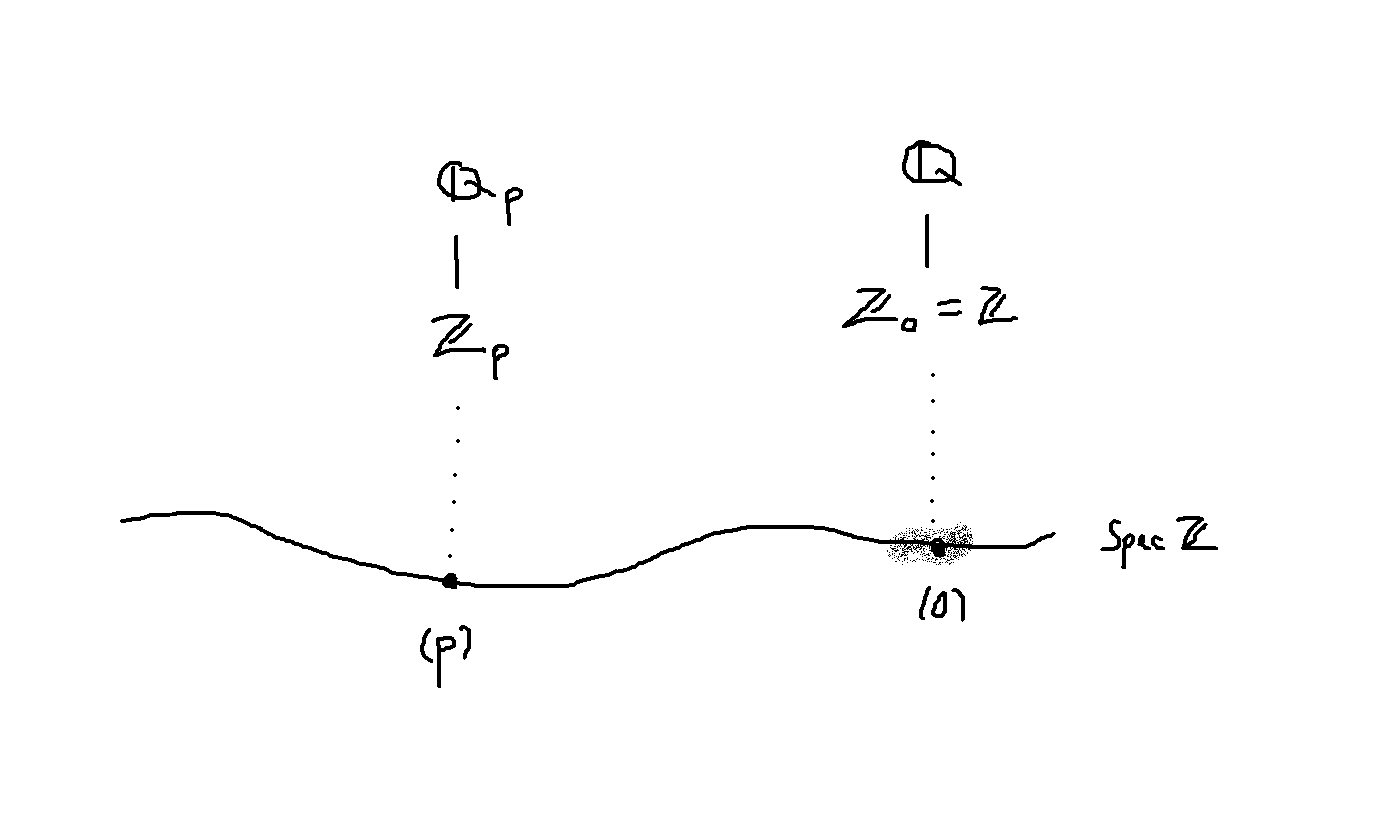
\includegraphics[width=\linewidth,height=\textheight,keepaspectratio]{Figures/places of Spec Z.png}
                                \caption{Local and global points of $\Spec \Z$}
                                \label{fig: local_and_global_points_of_Spec_Z}
                            \end{figure}
                    \end{remark}
                    \begin{definition}[Global models] \label{def: global_models}
                        We want our parametrising scheme, like $\Spec \Z$, to be one where the infinitestimal neighbourhoods (i.e. formal completions) around correspond to spectra of complete discrete valuation rings (for instance, the infinitestimal neighbourhoods $\Spf \Z_p$ around the points $(p) \in |\Spec \Z|$ correspond uniquely to the affine schemes $\Spec \Z_p$), which essentially means we want . We also want $S$ to be connected so that any residue field at a generic point would automatically be the function field of $S$.
                        
                        Let $S$ be base scheme satisfying the above conditions and let $K_0$ be its function field. Then, a \textbf{global model} for an algebraic scheme $X_0$ over $K_0$ shall be a flat and of finite type $S$-scheme $\bbX_0 \to S$. 
                    \end{definition}
                    \begin{remark}[Local-global compatibility] \label{remark: global_to_local_for_models}
                        
                    \end{remark}
                    
                    \begin{definition}[Pointed curves] \label{def: pointed_curves}
                        A \textbf{pointed elliptic curve} is a \textit{finitely presented} and \textit{proper} global model:
                            $$\bbE_0 \to S$$
                        with a distinguised so-called unit section $o_{\bbE_0}: S \to \bbE_0$ of one of the following:
                            \begin{itemize}
                                \item an elliptic curve over a place of $S$,
                                \item a projective nodal cubic curve over a place of $S$ (cf. \cite[\href{https://stacks.math.columbia.edu/tag/0C46}{Tag 0C46}]{stacks}), or
                                \item a projective cuspidal cubic curve over a place of $S$ (a point is a cusp if it corresponds to a non-splitting prime with inertial degree $2$; cf. definition \ref{def: ramification_indices}). 
                            \end{itemize}
                        A fibre of the first kind is said to be over a place of \textbf{good reduction}, whereas fibres over places of the second and third kind are said to be of \textbf{bad reduction}, as one ends up with singularities at those places.
                    \end{definition}
                    
                \paragraph{The geometry of \texorpdfstring{$\calM_{1, 1}$}{}}
                    \begin{proposition}[Base-changing $\calM_{1, 1}$] \label{prop: base_changes_of_moduli_spaces_of_elliptic_curves}
                        Let $\phi: S_2 \to S_1$ be a morphism between two base schemes and let $(\calM_{1, 1})_{/S_1}$ be the  moduli spaces of elliptic curves over $S_1$. Then, there exists a moduli space of elliptic curves $(\calM_{1, 1})_{/S_2}$ fitting into the following pullback square of geometric stacks:
                            $$
                                \begin{tikzcd}
                                	{(\calM_{1, 1})_{/S_1}} & {(\calM_{1, 1})_{/S_1}} \\
                                	{S_2} & {S_1}
                                	\arrow[from=1-2, to=2-2]
                                	\arrow[from=1-1, to=2-1]
                                	\arrow["{\phi}", from=2-1, to=2-2]
                                	\arrow["{}", from=1-1, to=1-2]
                                	\arrow["\lrcorner"{anchor=center, pos=0.125}, draw=none, from=1-1, to=2-2]
                                \end{tikzcd}
                            $$
                    \end{proposition}
                        \begin{proof}
                            First of all, the pullback $(\calM_{1, 1})_{/S_2}$ is \textit{a priori} a geometric stack on $\Sch_{/S_2}$. Next, consider a pullback square of the following form in $\Sch_{/S_1}$ (i.e. a pullback between fibres of $(\calM_{1, 1})_{/S_1}$):
                                $$
                                    \begin{tikzcd}
                                    	{f_1^* E_1} & E \\
                                    	{B_1'} & {B_1}
                                    	\arrow["{f_1}", from=2-1, to=2-2]
                                    	\arrow[from=1-2, to=2-2]
                                    	\arrow[from=1-1, to=1-2]
                                    	\arrow[from=1-1, to=2-1]
                                    	\arrow["\lrcorner"{anchor=center, pos=0.125}, draw=none, from=1-1, to=2-2]
                                    \end{tikzcd}
                                $$
                            along with a base change diagram of the following form:
                                $$
                                    \begin{tikzcd}
                                    	&& {B_2} & {B_1} \\
                                    	{B_2'} & {B'_1} & {S_2} & {S_1} \\
                                    	{S_2} & {S_1}
                                    	\arrow["\phi", from=3-1, to=3-2]
                                    	\arrow[from=2-2, to=3-2]
                                    	\arrow[from=2-1, to=2-2]
                                    	\arrow[from=2-1, to=3-1]
                                    	\arrow["\lrcorner"{anchor=center, pos=0.125}, draw=none, from=2-1, to=3-2]
                                    	\arrow["\phi", from=2-3, to=2-4]
                                    	\arrow[from=3-2, to=2-4]
                                    	\arrow[from=3-1, to=2-3]
                                    	\arrow["{f_2}", from=2-1, to=1-3]
                                    	\arrow["{f_1}", from=2-2, to=1-4]
                                    	\arrow[from=1-3, to=1-4]
                                    	\arrow[from=1-4, to=2-4]
                                    	\arrow[from=1-3, to=2-3]
                                    	\arrow["\lrcorner"{anchor=center, pos=0.125}, draw=none, from=1-3, to=2-4]
                                    \end{tikzcd}
                                $$
                            Pulling the first diagram back along $\phi: S_2 \to S_1$ (using the second diagram as a guide in the process) thus yields:
                                $$
                                    \begin{tikzcd}
                                    	{\phi^* f_1^* E_1} & {\phi^*E_1} \\
                                    	{B_2'} & {B_2} & {f_1^* E_1} & {E_1} \\
                                    	&& {B'_1} & {B_1}
                                    	\arrow[from=2-1, to=3-3]
                                    	\arrow["{f_2}", from=2-1, to=2-2]
                                    	\arrow["{f_1}", from=3-3, to=3-4]
                                    	\arrow[from=2-2, to=3-4]
                                    	\arrow[from=2-4, to=3-4]
                                    	\arrow[from=1-2, to=2-2]
                                    	\arrow[from=1-2, to=2-4]
                                    	\arrow[from=2-3, to=2-4]
                                    	\arrow[from=2-3, to=3-3]
                                    	\arrow[from=1-1, to=2-1]
                                    	\arrow[from=1-1, to=1-2]
                                    	\arrow[from=1-1, to=2-3]
                                    	\arrow["\lrcorner"{anchor=center, pos=0.125}, draw=none, from=2-3, to=3-4]
                                    	\arrow["\lrcorner"{anchor=center, pos=0.125}, draw=none, from=1-1, to=2-2]
                                    \end{tikzcd}
                                $$
                            We know \textit{a prioi} that $f_1* E_1$ and $\phi^* f_1* E_1$ must be elliptic curves, and with this, the proof is done.
                        \end{proof}
                    
                    \begin{proposition}[$\calM_{1, 1}$ is a geometric stack] \label{prop: moduli_stacks_of_elliptic_curves}
                        Let $S$ be a base scheme. Then, the moduli space of elliptic curves $(\calM_{1, 1})_{/S}$ is a geometric stack on $\Sch_{/S, \tau}$, where:
                            $$\tau \in \{\text{Zariski, \'etale, fppf, fpqc}\}$$
                        is a Grothendieck topology on $\Sch_{/S}$.
                    \end{proposition}
                        \begin{proof}
                            We will take definition \ref{def: schemes} as our working definition of schemes. It will become clear in a moment why this is necessary.
                            \begin{enumerate}
                                \item \textbf{(Descent satisfaction):} The sheaf condition (up to invertible $2$-cells, of course) is an easy consequence of the fact that pullbacks of elliptic curves along arrows $f: B \to B'$ in $\Sch_{/S}$ are given by fibred products (cf. definition \ref{def: moduli_of_elliptic_curves}).
                                \item \textbf{(A smooth atlas):} 
                                \item \textbf{(Schematicity of the diagonal):} 
                            \end{enumerate}
                        \end{proof}
            
            \subsubsection{Moduli of higher-dimensional abelian varieties}